\documentclass[a4paper,12pt]{article}
\usepackage[utf8]{inputenc}
\usepackage{graphicx}
\usepackage{geometry}  % Para ajustar los márgenes
\usepackage[hidelinks]{hyperref}
\usepackage{tikz}        % Carga el paquete TikZ
\usepackage{fancyhdr}  % Para personalizar el encabezado y pie de página
\usepackage{newtxtext,newtxmath}  % Paquetes para la fuente Times New Roman

\hyphenpenalty=10000  % Evita el guionado automático de palabras
\exhyphenpenalty=10000  % Evita guionar en palabras compuestas

% Configuración de los márgenes
\geometry{
    left=2.5cm,
    right=2.5cm,
    top=3cm,
    bottom=3cm,
}

\pagestyle{fancy}
\fancyhf{}
\fancyhead[L]{Programación de Aplicaciones Móviles Nativas}
\fancyhead[R]{Informe sobre Accesibilidad}
\fancyfoot[L]{}
\fancyfoot[R]{\thepage}
\renewcommand{\headrulewidth}{0.4pt}
\renewcommand{\footrulewidth}{0.4pt}

\begin{document}

\begin{titlepage}
    \centering
    % Incluye la imagen como portada
    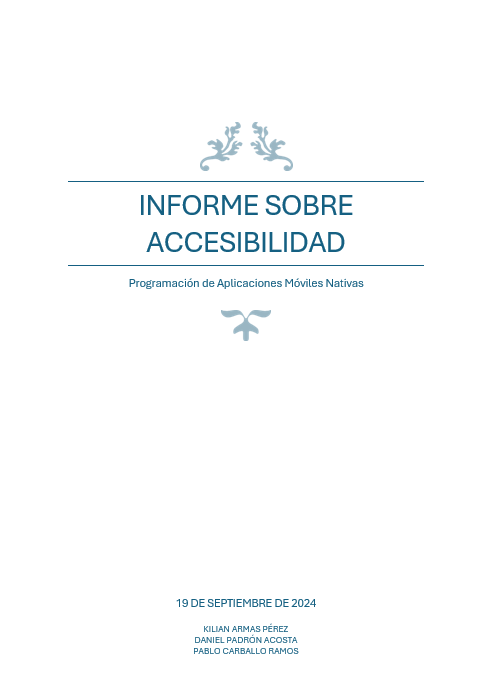
\includegraphics[width=\textwidth]{Images/portada.png}
\end{titlepage}

\newpage

\renewcommand{\contentsname}{Índice}

\tableofcontents

\newpage

\section{Introducción}
En este informe se analizará la accesibilidad de la página web oficial de Guaguas Global y de la aplicación móvil de Guaguas Municipales. Las guaguas son un servicio esencial, especialmente para aquellas personas con discapacidades que les impidan conducir, por lo que nos ha parecido relevante analizar el nivel de accesibilidad que presentan. 

Para ello, primero realizaremos un análisis personal del sitio web de Global, teniendo como referencia los 4 principios de la accesibilidad (WCAG): perceptible, operable, comprensible y robusto. Tras esto, emplearemos algunas herramientas externas que analizarán la accesibilidad y compararemos los resultados. Finalmente, analizaremos la aplicación móvil de Guaguas Municipales en términos de accesibilidad.

\vspace{2cm}

\hspace{-0.5cm}

\includegraphics[width=0.4\textwidth]{Images/global.png}
\hspace{0.5cm}

\includegraphics[width=0.55\textwidth]{Images/guaguas_municipales.png}

\newpage

\section{Análisis personal del sitio web de Global}

\subsection{Landing Page}

\textbf{Navegación:} El menú principal no es completamente accesible mediante teclado, lo que dificulta su uso para personas con discapacidades motoras.\\
\textbf{Imágenes:} Algunas imágenes carecen de texto alternativo adecuado, afectando a los usuarios de lectores de pantalla.\\
\textbf{Contraste:} Problemas de contraste en elementos clave, como el banner principal, dificultan la legibilidad.

\vspace{0.3cm}
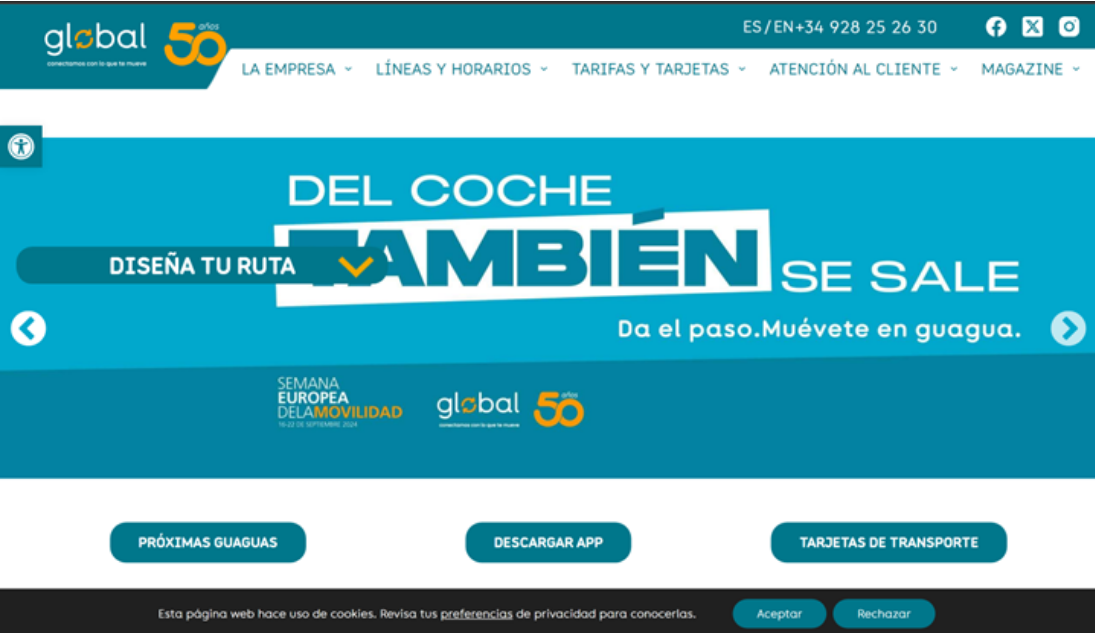
\includegraphics[width=0.8\textwidth]{Images/global_landing_page.png}

\subsection{Sección de Horarios}
\textbf{Información visual:} Gráficos y tablas carecen de descripciones textuales, lo que afecta a los usuarios con discapacidades visuales.

\vspace{0.3cm}
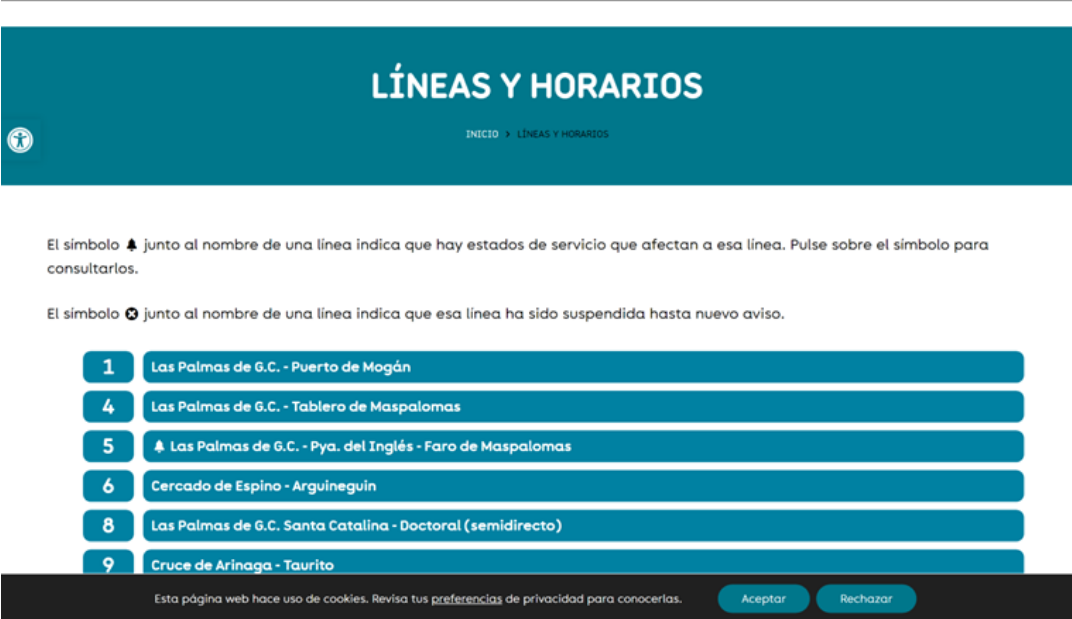
\includegraphics[width=0.8\textwidth]{Images/global_horarios.png}

\newpage

\subsection{Sección de Tarifas}
\textbf{Legibilidad:} El contraste en algunos textos no cumple con los estándares de WCAG (nivel AA), afectando a personas con problemas de visión.\\
\textbf{Escalabilidad:} Al aumentar el tamaño del texto, algunos elementos se desorganizan o no se ajustan correctamente.

\vspace{0.3cm}
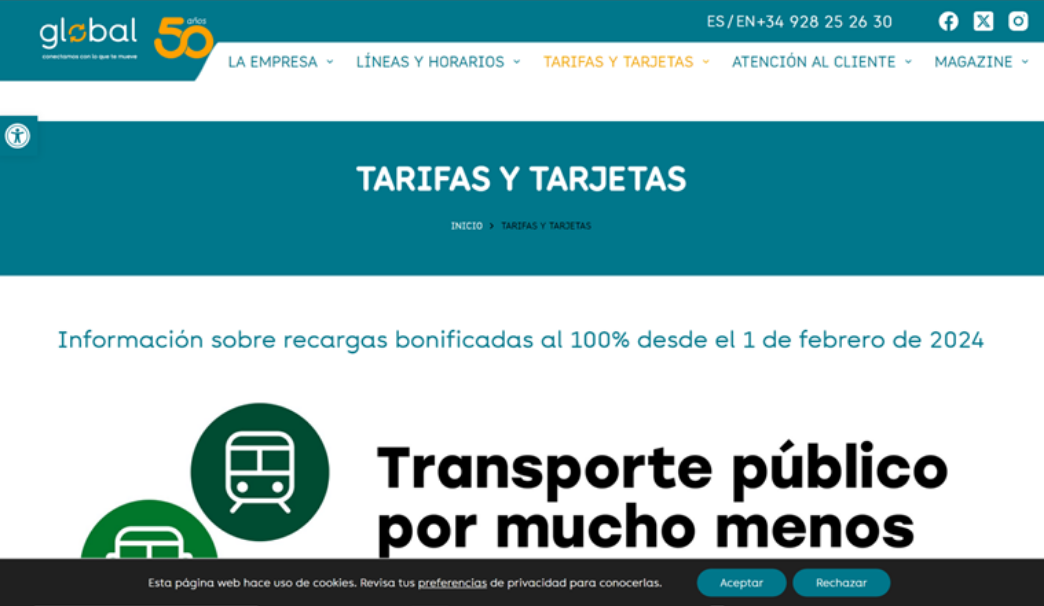
\includegraphics[width=0.8\textwidth]{Images/global_tarifas.png}

\subsection{Sección de Contacto}
\textbf{Mapas interactivos:} Los mapas no ofrecen alternativas accesibles, complicando su uso para personas con discapacidades visuales.\\
\textbf{Captchas:} Si están presentes, no parecen ofrecer una alternativa accesible para personas con discapacidades cognitivas o visuales.

\vspace{0.3cm}
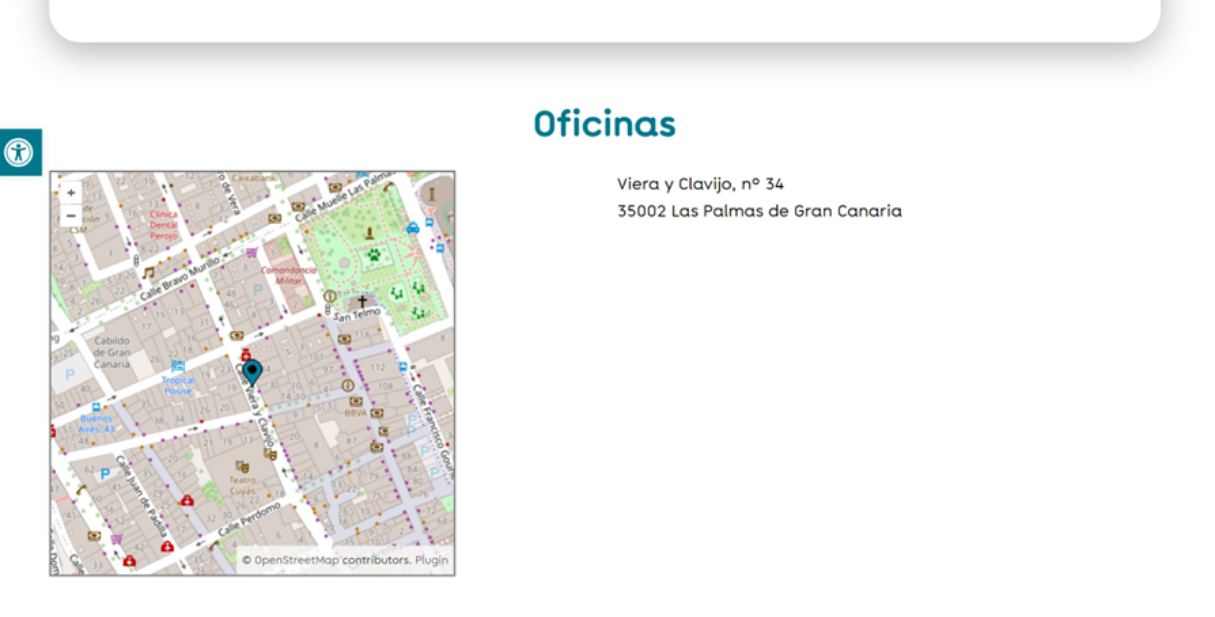
\includegraphics[width=0.8\textwidth]{Images/global_contacto.png}

\vspace{-0.5cm}
\subsection{Conclusión}
El sitio presenta varios problemas de accesibilidad que afectan su uso para personas con discapacidades, según las pautas WCAG. Se recomienda mejorar el contraste, la navegación por teclado, el uso de textos alternativos y la accesibilidad de formularios y mapas.

\newpage

\section{Comparativa entre el informe con Lighthouse y nuestro análisis}
Hemos realizado una comparación entre nuestro análisis de la página de Guaguas Global y los resultados obtenidos por Lighthouse.

\subsection{Overview de Lighthouse}

\vspace{0.3cm}
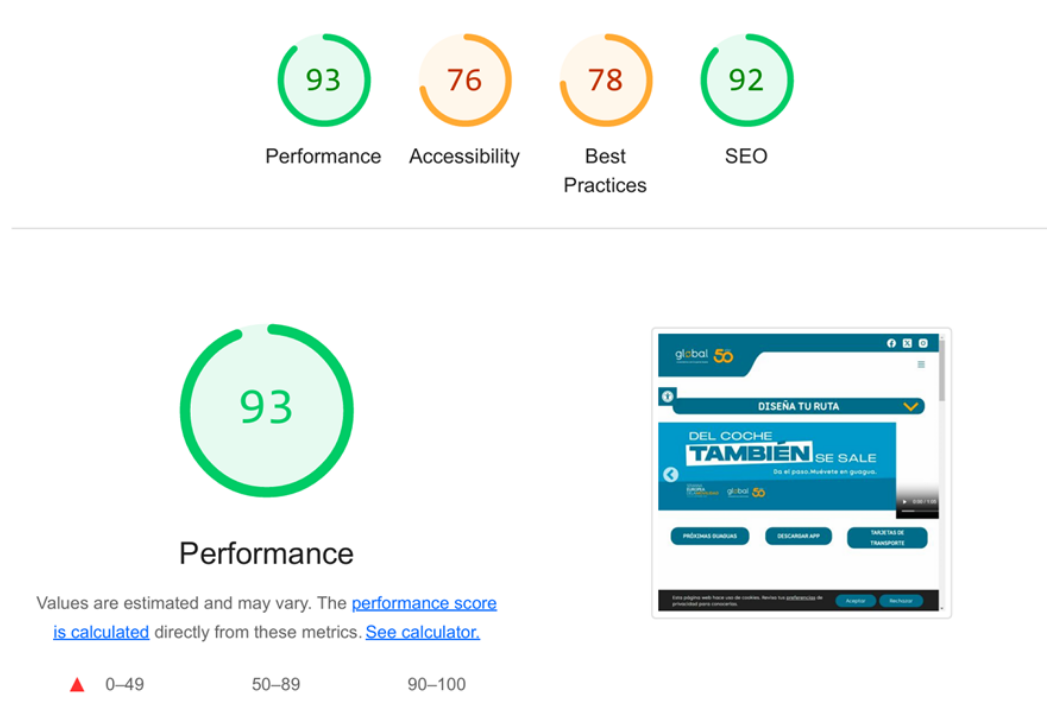
\includegraphics[width=0.8\textwidth]{Images/overview_lighthouse.png}

\subsection{Navegación y Accesibilidad}
En nuestro análisis, mencionamos que el menú principal no es completamente accesible mediante teclado, lo que dificulta su uso para personas con discapacidades motoras. Lighthouse también detecta problemas de navegación, como elementos que no están en el orden correcto para navegar con el teclado y títulos que no siguen una secuencia lógica, lo que afecta la experiencia de los usuarios que dependen de estas tecnologías.

\vspace{0.3cm}
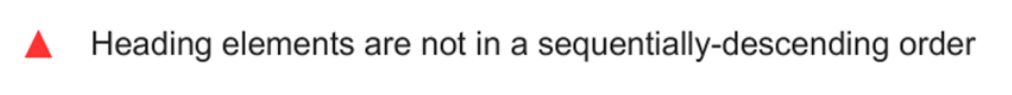
\includegraphics[width=0.8\textwidth]{Images/navegacion_accesibilidad.png}

\vspace{-0.2cm}
\subsection{Texto Alternativo y Contraste}
Identificamos que hay problemas de contraste en ciertos elementos que dificultan la lectura. Lighthouse también resalta los problemas de contraste, afectando la legibilidad del contenido.

\vspace{0.3cm}
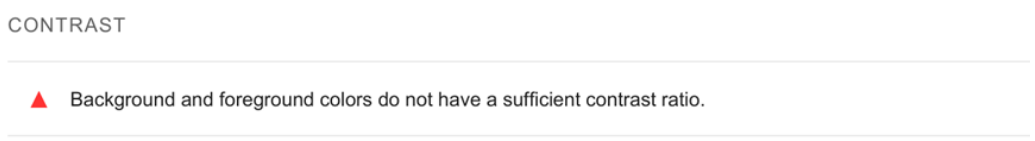
\includegraphics[width=0.8\textwidth]{Images/texto_contraste.png}

\newpage

\subsection{Formularios y Campos de Entrada}
Observamos que los formularios no tienen etiquetas visibles, lo que hace que los lectores de pantalla no puedan interpretarlos correctamente. Lighthouse sugiere mejorar los controles y la estructura semántica para hacer estos elementos más accesibles.

\subsection{Gráficos y Tablas}
En nuestro análisis, mencionamos la falta de descripciones en gráficos y tablas, lo que afecta a los usuarios con discapacidades visuales. Lighthouse recomienda realizar revisiones manuales para evaluar contenidos multimedia.

\subsection{Mapas y Captchas}
Notamos que los mapas interactivos no tienen alternativas accesibles y que los captchas pueden presentar barreras para personas con discapacidades visuales o cognitivas. Lighthouse resalta la importancia de tener contenido alternativo para multimedia, lo cual también se aplica a los mapas.

\subsection{Conclusión sobre los Cambios Prioritarios}
Tanto nuestro análisis como el de Lighthouse coinciden en que los principales problemas de accesibilidad de la página se encuentran en la navegación, la falta de texto alternativo y los problemas de contraste. Las mejoras recomendadas son:

\begin{enumerate}
    \item Mejorar el contraste en los elementos principales para que sean más legibles.
    \item Añadir texto alternativo a las imágenes para que los usuarios con lectores de pantalla puedan entender el contenido visual.
    \item Optimizar la navegación por teclado corrigiendo la jerarquía de los títulos y ajustando los elementos interactivos.
    \item Hacer los formularios más accesibles con etiquetas y descripciones claras.
\end{enumerate}

\newpage

\section{Análisis de la aplicación móvil Guaguas Municipales}
\subsection{Sección principal}
Observamos una interfaz con un diseño claro e intuitivo, con iconos que indican su función y con una buena distribución. Además,  dichos botones tienen colores contrastantes, muy útil para personas con alguna dificultad visual.

\begin{figure}[htbp]
    \centering
    \begin{minipage}{0.5\textwidth}
        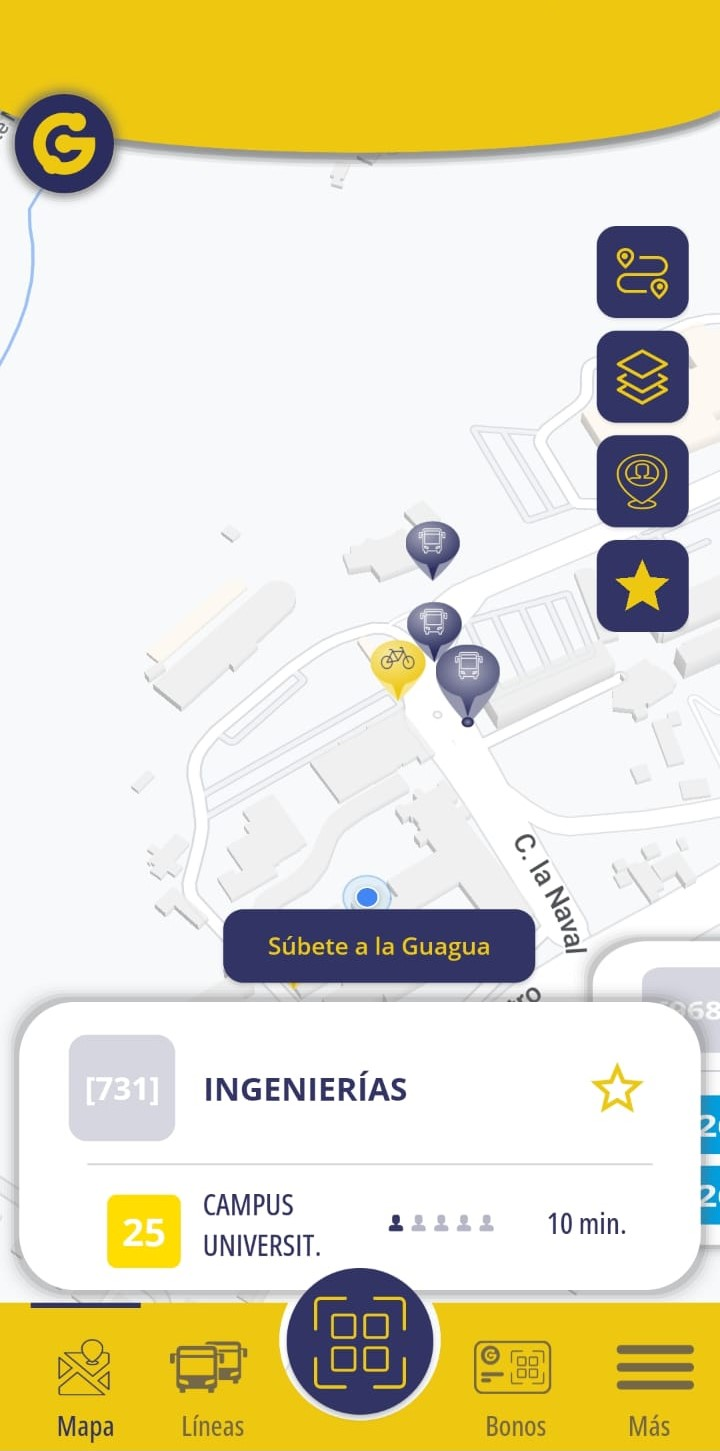
\includegraphics[width=\linewidth]{Images/seccion_principal.jpg}
    \end{minipage}%
    \hspace{0.8cm}
    \begin{minipage}{0.3\textwidth}
        \setlength{\parskip}{20pt}  % Espacio entre párrafos de 10 puntos
        
        Las paradas presentes en el mapa son claras y éste se puede ampliar, ayudando así a ciertas personas con dificultades a seleccionar la que deseen correctamente.
        
        En cuanto a la sección de las paradas, se muestra aquella información esencial para los usuarios.
        
        La aplicación está diseñada para soportar texto alternativo, por lo que las personas con ciertas discapacidades visuales podrán hacer uso de la misma con normalidad.
        
        Como punto negativo, el amarillo brillante y el blanco pueden ser confundidos por usuarios con algún tipo de daltonismo.
        
        Por otro lado, se podría espaciar un poco más los botones situados a la derecha para facilitar el uso a ciertos usuarios.
    \end{minipage}
\end{figure}

\newpage

\subsection{Sección de líneas}
En esta sección, podemos apreciar que los colores asignados a cada línea de guagua son consistentes y ayudan a identificar rápidamente las rutas. Esto es útil para los usuarios frecuentes que pueden asociar un color a una ruta específica.

\begin{figure}[htbp]
    \centering
    \begin{minipage}{0.5\textwidth}
        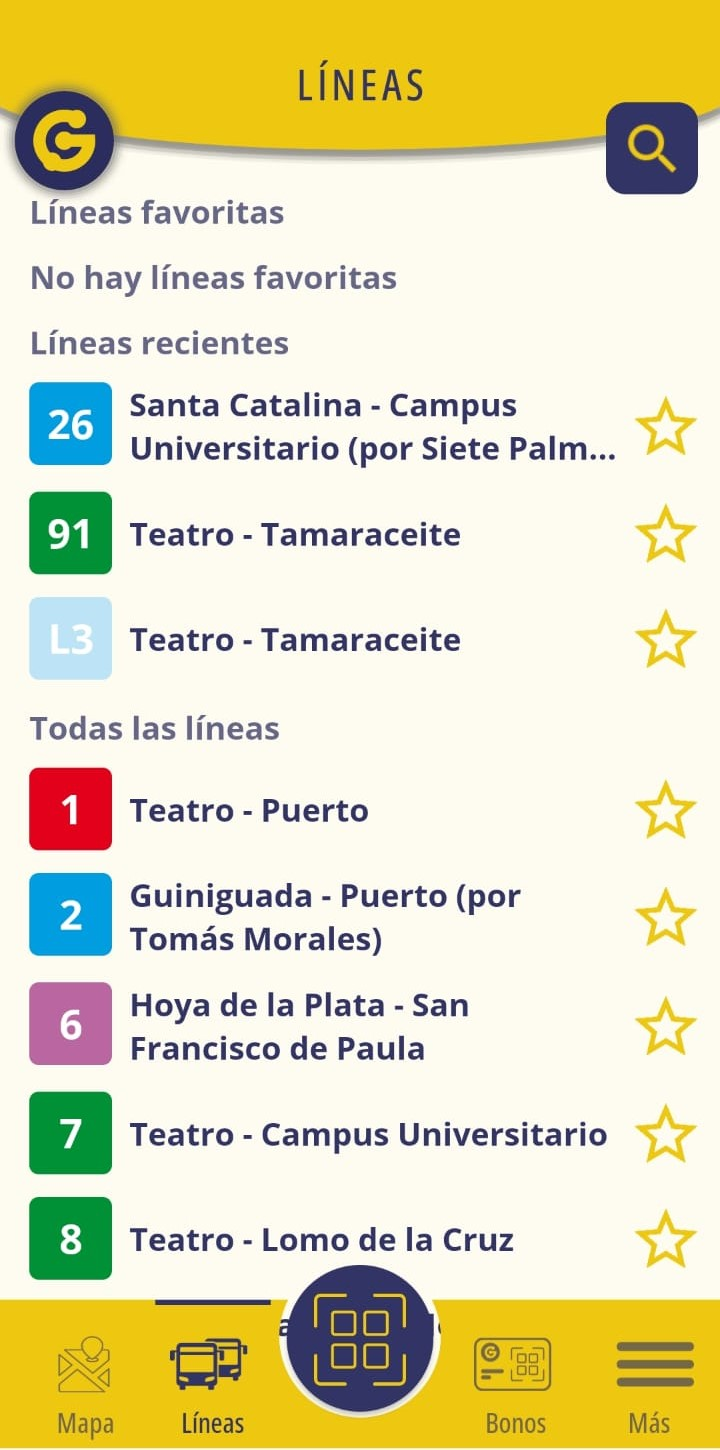
\includegraphics[width=\linewidth]{Images/seccion_lineas.jpg}
    \end{minipage}%
    \hspace{0.8cm}
    \begin{minipage}{0.3\textwidth}
        \setlength{\parskip}{20pt}  % Espacio entre párrafos de 10 puntos
        
        Además, el botón de búsqueda (lupa) en la parte superior derecha es fácil de identificar, permitiendo buscar otras líneas de manera rápida.
        
        A pesar de los detalles positivos anteriormente nombrados, algunos puntos de mejora podrían ser:

        \textbf{Texto truncado:} En el caso de algunas líneas, el texto está truncado. Esto podría generar confusión a los usuarios si no pueden ver toda la información relevante de una línea.
        
        \textbf{Jerarquía de información:} La pantalla presenta mucha información en un formato bastante comprimido.
    \end{minipage}
\end{figure}

\newpage

\subsection{Sección "Más"}
Las opciones principales de esta sección están bien categorizadas, lo que facilita a los usuarios encontrar rápidamente la funcionalidad que buscan. Y la disposición en lista vertical proporciona un diseño familiar y fácil de seguir para la mayoría de los usuarios.

\begin{figure}[htbp]
    \centering
    \begin{minipage}{0.5\textwidth}
        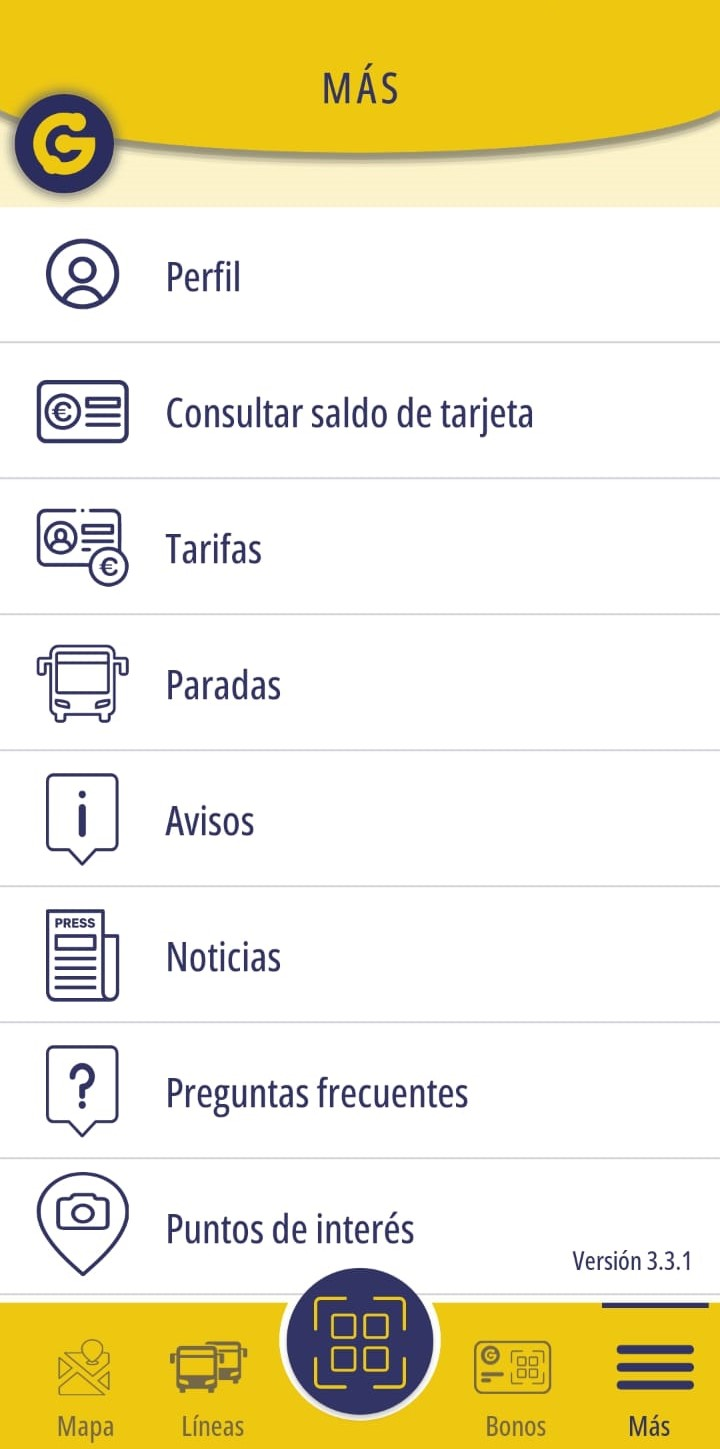
\includegraphics[width=\linewidth]{Images/seccion_mas.jpg}
    \end{minipage}%
    \hspace{0.8cm}
    \begin{minipage}{0.3\textwidth}
        
        \setlength{\parskip}{20pt}  % Espacio entre párrafos de 10 puntos
        
        También hay que remarcar que cada opción viene acompañada de un icono, lo cual es útil para los usuarios, ya que agrega contexto visual y hace la navegación más intuitiva. Además, estos iconos son claros y reconocibles.

        Aunque en general, esta sección está bien organizada, el texto dentro de las opciones principales podría beneficiarse de un mayor espaciado entre líneas. Esto ayudaría a los usuarios a identificar cada opción más claramente y evitaría que el contenido se sienta amontonado.
    \end{minipage}
\end{figure}

\subsection{Conclusión sobre la aplicación móvil}
La aplicación móvil es funcional y está bien organizada, pero puede mejorar en términos de accesibilidad y jerarquía de información. Se recomiendan ajustes en los contrastes de color, espaciado y tamaño de los botones interactivos, además de mejoras en la estabilidad de la sesión del usuario.

\end{document}
